\section{Introduction}
So far at the LHC, no direct evidence for new physics has been observed with a significance greater than 5 standard deviations. It could be that the searches are not looking in the right direction, e.g.\ all that is needed is to search in a particular final state, or consider an exotic signature, like a long-lived particle, which are less commonly explored at the LHC. Alternatively, it could just be that the couplings in the new theory are small such that the new particles are produced at a rate that is too low to be observed with the current data set. Optimistically, one could then hope that the new particles are within reach at the end of the LHC's lifetime. 

However, it is also possible that the mass of the new particle is larger than the LHC energy reach, in which case, the only evidence of new physics provided by the LHC would be through indirect effects of new particles, which can be parameterized by the Wilson coefficients in an Effective Field Theory (EFT). The observation of a Wilson coefficient taking a non-zero value would be an indication of new physics, and the compatibility of that observation with BSM theories can be assessed via a procedure called \textit{matching}~\cite{Carmona:2021xtq} where the constraints on Wilson coefficients are translated into constraints on the parameters of a BSM theory.

The indirect effects predicted by an EFT can be seen in SM processes as a deviation in the higher-energy tail of a distribution, as illustrated in \cref{fig:eft_xkcd}, or as an overall scaling of processes, or even exceptionally, as a deviation in the lower-energy tails of a distribution, as in the case of the \Hfl decay discussed in \cref{sec:h4l_eft_theory}. Therefore, indirect hints of new physics could be present in the large variety of SM measurements already made at the LHC. Furthermore, under a common EFT framework, measurements can be combined to provide better sensitivity to new physics than possible with a standalone analysis.  

\begin{figure}
  \centering
  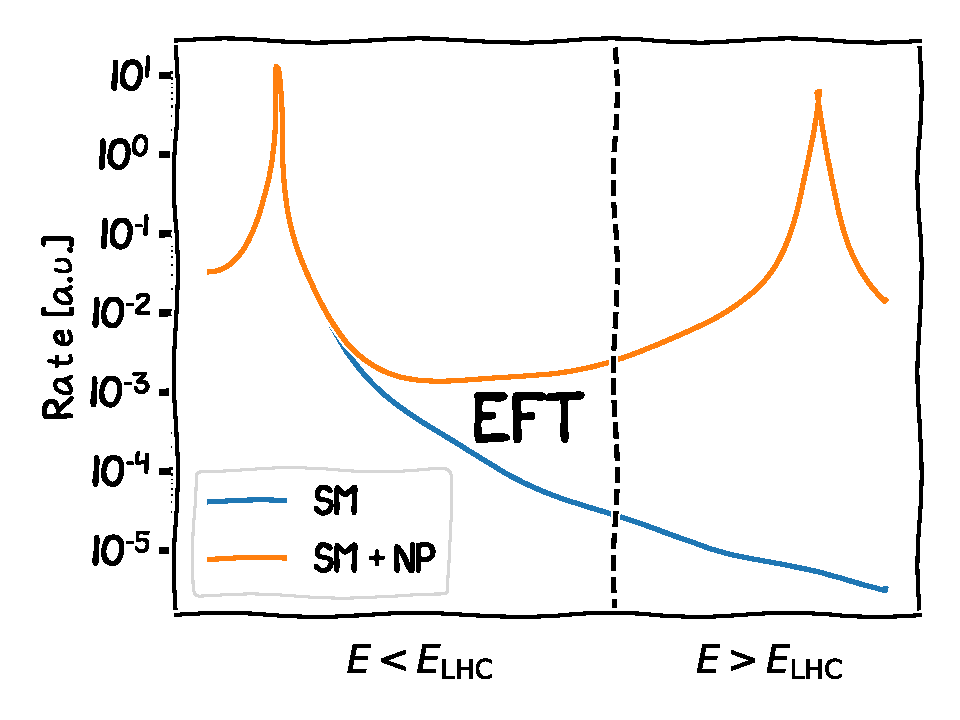
\includegraphics[width=0.6\textwidth]{Figures/EFT/xkcd.pdf}
  \caption[Illustration of EFT Effects in High-Energy Tails of Distributions]{Toy examples of invariant mass distributions, one which is from a SM resonance (blue), and another that also includes a new resonance (orange). The dashed line indicates the boundary of the LHC's energy reach which is $\mathcal{O}(1\TeV)$. Given that the new resonance is beyond that line, its direct detection would not be possible at the LHC, but its indirect effects, which are visible to the left of the dashed line, could be detected. Such an effect is predicted by EFTs and could be detected in an EFT interpretation.}\label{fig:eft_xkcd}
\end{figure}

This chapter presents an SMEFT (\cref{sec:EFT}) interpretation of a combination of Higgs boson analyses that use data collected by the CMS experiment during proton-proton collisions at $\sqrtS=13$\TeV between 2016 and 2018, corresponding to an integrated luminosity of 138\fbinv~\cite{CMS-PAS-HIG-21-018}. This is the same combination that reported the STXS results discussed in \cref{sec:stxs}. The input analyses, summarized in \cref{tab:eft_input_channels}, measure the rate of Higgs boson production in an exhaustive variety of decay channels and production modes. Their combination allows for the isolation of new physics effects to specific production or decay modes, and even to specific kinematic regions within those modes, thanks to the inclusion of the STXS (\cref{sec:higgs_pheno}) binning in most of the analyses. In an EFT framework, this corresponds to the possibility to simultaneously constrain a good number of Wilson coefficients. 

\begin{table}
    \centering
    \caption[Summary of the Analyses in the Combination Used for the SMEFT Interpretation]{Summary of the analyses in the combination used for the SMEFT interpretation. Analyses target particular final states and one or more production modes which are indicated by the production tags. In some analyses, the measurement of particular production modes is split according to the stage 1.2 STXS. This is indicated by a checkmark in the final column, and the corresponding splitting is described in the production tags. For example, the \Hgg analysis measures the \ttH production mode in \pt bins, as shown in \cref{fig:stxs_stage1p2_results}, whereas the \Hfl analysis measures this mode inclusively.}
    \centering
    \renewcommand{\arraystretch}{1.2}
        \begin{tabular}{c|c|l|c}\hline
            Input analysis                        & Final states                                                                                                        & Production tags                                                                                                                                                                                          & Stage 1.2         \\ \hline
            \Hgg~\cite{CMS:2021kom}               & $\gamma\gamma$                                                                                                      & \begin{tabular}{@{}l@{}}ggH, $p_T^H$ x N-jet + BSM bins \\ VBF, $m_{jj}$ x $p_T^{Hjj}$ + BSM bins \\ VH hadronic \\ WH leptonic, $p_T^V$ bins \\ ZH leptonic \\ ttH, $p_T^H$ bins \\ tH \end{tabular}    & \checkmark        \\ \hline
            \Hfl~\cite{CMS:2021ugl}               & 4$\mu$, 2e2$\mu$, 4e                                                                                                & \begin{tabular}{@{}l@{}}ggH, $p_T^H$ x N-jet + BSM bins \\ VBF, $m_{jj}$ x N-jet + BSM bins \\ VH hadronic \\ VH leptonic, $p_T^V$ bins \\ ttH\end{tabular}                                              & \checkmark        \\ \hline
            \Hlnulnu~\cite{CMS:2022uhn}           & \begin{tabular}{@{}c@{}}e$\mu$/$\mu$e, ee+$\mu\mu$ \\ e$\mu$+jj, 3$l$, 4$l$\end{tabular}                            & \begin{tabular}{@{}l@{}}ggH, $p_T^H$ x N-jet + BSM bins \\ VBF-like $m_{jj}$ + BSM bins \\ VH hadronic \\ WH leptonic \\ ZH leptonic\end{tabular}                                                        & \checkmark        \\ \hline
            \Htautau~\cite{CMS:2022kdi}           & \begin{tabular}{@{}c@{}}e$\mu$, e$\tau_h$, $\mu\tau_h$ \\ $\tau_h\tau_h$\end{tabular}                               & \begin{tabular}{@{}l@{}}ggH, $p_T^H$ x N-jet + BSM bins \\ VBF, $m_{jj}$ x N-jet + BSM \\ WH leptonic, $p_T^V$ bins \\ ZH leptonic, $p_T^V$ bins\end{tabular}                                            & \checkmark        \\ \hline
            \Hbb boosted~\cite{CMS:2024ddc}       & bb                                                                                                                  & \begin{tabular}{@{}l@{}}ggH, high $p_T^H$ bins \\ VBF, high $p_T^H$ bins\end{tabular}                                                                                                                    & \checkmark        \\ \hline
            VBF, \Hbb~\cite{CMS:2023tfj}          & bb                                                                                                                  & VBF, resolved                                                                                                                                                                                            &                   \\ \hline
            VH, \Hbb~\cite{CMS:2023vzh}           & bb                                                                                                                  & \begin{tabular}{@{}l@{}}WH leptonic, $p_T^V$ bins \\ ZH leptonic, $p_T^V$ bins\end{tabular}                                                                                                              & \checkmark        \\ \hline
            ttH, \Hbb~\cite{CMS:2024fdo}          & bb                                                                                                                  & \begin{tabular}{@{}l@{}}ttH, $p_T^H$ bins \\ tH\end{tabular}                                                                                                                                             & \checkmark        \\ \hline
            ttH multilepton~\cite{CMS:2020mpn}    & \begin{tabular}{@{}c@{}}2$l$(ss), 3$l$, 4$l$ \\ 1$l$+2$\tau_h$, 2$l$(ss)+1$\tau_h$ \\ 3$l$+1$\tau_h$\end{tabular}  & ttH, tH                                                                                                                                                                                                   & \checkmark        \\ \hline
            \Hmumu~\cite{CMS:2020xwi}             & $\mu\mu$                                                                                                           & ggH, VBF, VH, ttH                                                                                                                                                                                         &                   \\ \hline
            \HZg~\cite{CMS:2022ahq}               & $l^+l^-\gamma$                                                                                                     & ggH, VBF                                                                                                                                                                                                  &                   \\
        \end{tabular}\label{tab:eft_input_channels}
\end{table}

The parameterization of these measurements in terms of the Wilson coefficients, described in \cref{sec:eft_parameterization}, is determined partly with the provision of analytically-derived equations, and mostly via the use of MC-based techniques. The methodology improves upon the previous iteration of this combination performed by the CMS experiment~\cite{CMS:2020gsy} in a number of ways, most notably, by calculating the \ggH and \ggZH predictions at loop-level, introducing propagator corrections, and including acceptance corrections for the \Hfl and \Hlnulnu decay channels.

The final results, provided in \cref{sec:eft_nominal_basis_results,sec:eft_rotated_basis_results}, are presented in two ways. First, 68\% and 95\% CL constraints on individual Wilson coefficients are shown, where the other coefficients are set to their SM values of zero. These results are sensitive to very specific types of new physics signatures (related to just one Wilson coefficient). However, it is expected that a BSM theory would lead to non-zero values of multiple Wilson coefficients. Therefore, simultaneous constraints on multiple Wilson coefficients are also extracted. In these results, a rotated basis for the Wilson coefficients is used to determine the constraints, where the rotated basis is determined via a principal component analysis (PCA). 